\documentclass{article}  % Document class (can be article, report, book, etc.)

% Preamble: add packages here (optional)
\usepackage[utf8]{inputenc}  % Ensures proper encoding
\usepackage{amsmath}  % Math symbols package (optional)
\usepackage{graphicx} % Allows inclusion of images (optional)

\parindent 0mm
\linespread{1.25}

\title{Digitales Wahlsystem}
\author{
    Muhamedbaqir Al-Rumeil \and 
    Tizian Grossmann \and 
    Leon Meier
    }

\date{\today}  % Can be \today for today's date for a specific date

\begin{document}
\pagenumbering{roman}

\maketitle
\newpage

\tableofcontents
\newpage

\pagenumbering{arabic}
\section{Anforderungen an verteilte Systeme}

Heutzutage werden viele Softwarelösungen nach einer verteilten Architektur gerichtet, um Use-Case spezifische Anforderungen besser (oder überhaupt) erfüllen zu können. \\
Die Anforderungen an eine Lösung und die Herausforderungen einer möglichen verteilten Architektur sind immer spezifisch, mögliche Anforderungen wären: Ausfallsicherheit, geringe Latenzen, Datenredundanz, etc.  \\

Es ist wichtig zu erkennen, dass die Architektur nicht willkürlich alle möglichen Ziele erfüllen kann, sondern sich nach dem zugrunde liegenden Problem richten sollte. In einem ERP-System hat die Latenz beispielsweise nicht den selben Stellenwert wie in einem autonomen Fahrsystem. \\
Es bedarf also immer einer gründlichen Analyse der Anforderungen, um die Architektur sinnvoll umsetzen zu können. \\


Dieses Paper befasst sich mit der Planung und Implementation eines Wahlsystems, welches die deutsche Bundestagswahl, mitsamt Erst- und Zweitstimme abbilden soll. Unser Ziel ist es, ein verteiltes System zu definieren, welches eine hohe Verfügbarkeit und gute horizontale Skalierbarkeit aufweist.
  
\newpage

\section{Ablauf einer Bundestagswahl}
Der analoge Ablauf einer Bundestagswahl ist gesetzlich definiert und erlaubt unserem digitalem Wahlsystem keinen Spielraum. Folgendes Diagramm beschreibt (vereinfacht) den Prozess, den wir digitalisieren wollen. \\

\begin{figure}[h] % 'h' means place the figure here
    \centering % Center the image
    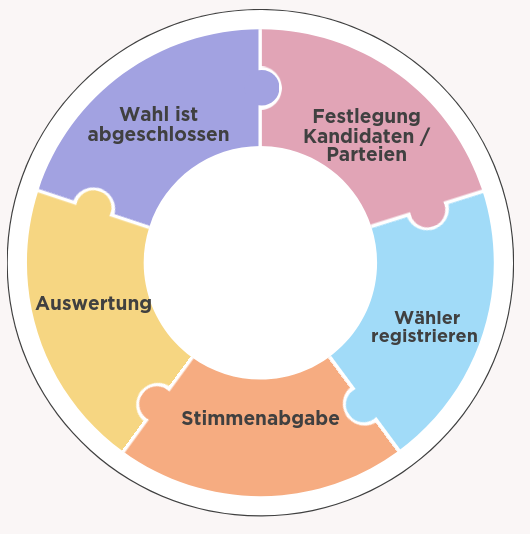
\includegraphics[width=0.8\textwidth]{election_process} % Adjust width to 50% of text width
    \label{fig:example} % Add a label for referencing
\end{figure}

Aus dem Ablauf der Wahl kristallisieren die wichtigsten Anforderungen: \\
\begin{itemize}
    \item Viele Schreiboperationen: Die größte Last auf die Datenbank(en) wird das Einfügen der Stimmen sein. Die Leseoperationen (Kandidaten, Parteien, Wahlkreise) sind während der Wahl statisch und das Auswerten (ebenfalls eine Leseoperation) geschieht nur einmalig zum Ende einer Wahl. 

    \item Eventuelle Konsistenz: Die Stimmen werden erst alle gesammelt und im Anschluss ausgewertet. Es reicht also aus Schreiboperationen vorzumerken, anstatt direkt auszuführen. \\ Erst, wenn die Stimmen ausgewertet werden sollen, muss der Zustand der eventuellen Konsistenz eintreten.

    \item Ausfallsicherheit: Wie anfangs festgelegt, muss das System ausfallsicher sein und keinen einzigen Ausfallpunkt besitzen dürfen. Die Wählerstimmen dürfen also nicht an einem einzigen Ort gespeichert sein, und es darf nicht über eine einzige Instanz mit den Daten interagiert werden. \\
    Wir brauchen also ein redundantes und ständig verfügbares System.


    \item Partitionierung: Da ein Wähler nicht mehrmals wählen darf, kann die Datenstruktur nicht nach Wahlkreis, Partei oder Kandidaten partitioniert sein, da dies bei vielen Schreiboperationen die Leistung drastisch reduzieren würde (aufgrund von Locks). Wären die Daten partitioniert, müsste man bei jeder Schreiboperation jede Partition abfragen, ob der vorliegende Eintrag gültig ist oder nicht. \\ Desweiteren bräuchte es für jede Partition mehrere Instanzen, welche die Daten redundant speichern, diese Daten müssten ebenfalls synchronisiert werden und man bräuchte eine weitere Instanz zur Lastverteilung und Verwaltung der Partitionsinstanzen. Alles in allem also ein sehr großer Aufwand.

 
\end{itemize} 

Wir fassen also zusammen, dass wir eine verteilte Datenbank brauchen, welche schnelle Schreibgeschwindigkeiten unterstützt und die Daten nicht partitioniert werden. \\
Desweiteren brauchen wir mehrere Backend Intanzen, welche mit der verteilten Datenbank interagieren. \\

\newpage
\section{Cassandra}
An dieser Stelle würde üblicherweise erst die Architektur eruiert werden, anstatt auf eine konkrete Technologie einzugehen. \\
Jedoch sind die eben ermittelten Anforderungen so passend, dass es nur Sinn ergibt die Auswahl der Datenbanktechnologie, nämlich Cassandra, zu erklären.\\

Cassandra ist ein verteilter nicht-relationaler Column Store, welcher aus den folgenden Gründen die beste Lösung für den Use-Case unserer Bundestagswahl ist.\\

    \begin{tabular}{  p{0.3\linewidth} | p{0.8\linewidth} }
        Anforderung & Cassandra Funktion\\ 
        \hline
     Schreibgeschwindigkeit 
        
     Eventuelle Konsistenz& Cassandra schreibt einen Insert nicht direkt auf die Festplatte, sondern schreibt ihn erst in den Hauptspeicher und inseriert ihn zum nächstmöglichen Zeitpunkt.

     \vspace{1em}

     Dies ist möglich durch die nicht-relationale Struktur, denn ein Insert über viele normalisierte Tabellen hinweg würde nur in ständigen Hardlocks resultieren.  
     
     \vspace{1em}
     Die Verzögerung bis zum Ausführen der Operationen im Hauptspeicher ist eben die eventuelle Konsistenz, welche für uns bedeutet, dass wir sehr viele Schreiboperationen abhandeln können.
     vgl. \cite{storage-engine}\\ 

     \hline
     Redundanz 
          
     Verfügbarkeit& 
     
      
    Cassandra bildet ein Cluster aus beliebig vielen Nodes, welche die Daten redundant speichern, zu einem frei wählbaren Duplizierungsgrad 
    
    \vspace{1em}

    Des Weiteren kann Cassandra dynamisch mit dem Hinzufügen und Entfernen von Nodes umgehen, ohne dass die Verfügbarkeit darunter leidet.

    Die Daten werden entsprechend dem Duplizierungsgrad auf die Nodes verteilt.
    
    \vspace{1em}
    
    Diese zwei Punkte bedeuten also, dass Cassandra die Daten hochverfügbar und dupliziert für unser Wahlsystem speichern kann.
    vgl. \cite{overview}
    \\

      \hline
      Partitionierung & 
      
      Alle Cassandra Nodes bilden einen Keyspace, vereinfacht gesagt eine logische Datenbank mit über allen Nodes gleichen Tabellen. 

      Für unser System ist das aufgrund der schwer möglichen Datenpartitionierung optimal.
      \cite{overview}
      \\   
    \end{tabular}
    \\
    Cassandra entspricht also unseren Ansprüchen an die Datenspeicherung und ist daher die Datenbanktechnologie unserer Wahl.
\newpage
\section{Architektur}
Wir entschieden Cassandra zur Datenspeicherung und Zustandsspeicherung zu benutzen, und dementsprechend richten wir den Rest des Wahlsystems danach. \\
Um horizontale Skalierbarkeit, hohe Verfügbarkeit und Ausfallsicherheit zu erreichen, gestalten wir unser Wahlsystem wie folgt: \\

\begin{figure}[h] % 'h' means place the figure here
    \centering % Center the image
    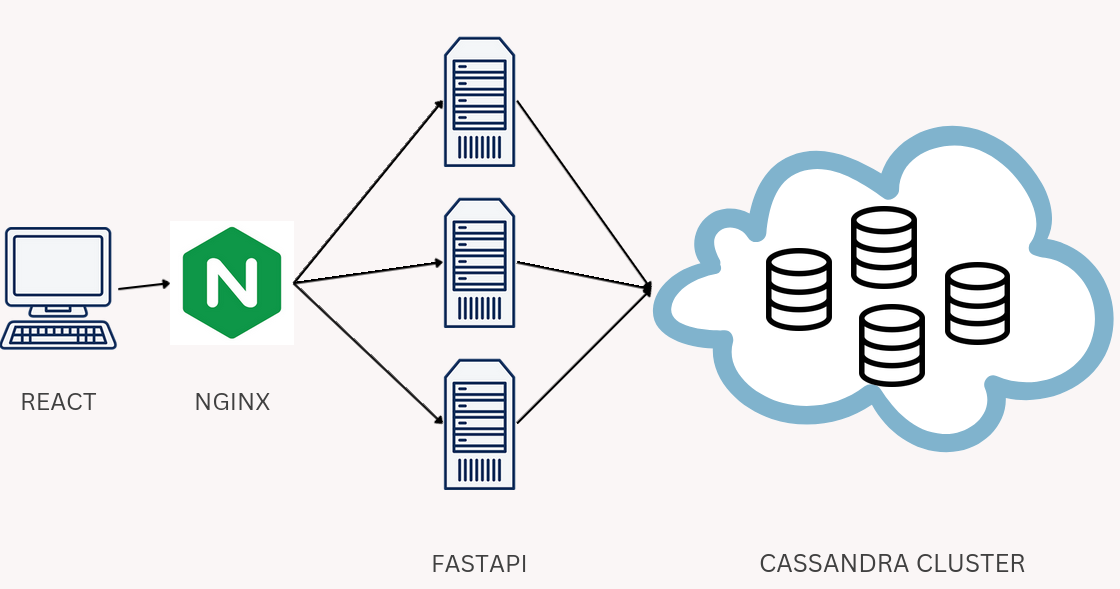
\includegraphics[width=0.8\textwidth]{architecture} % Adjust width to 50% of text width
    \caption{An example image.} % Add a caption
    \label{fig:example} % Add a label for referencing
\end{figure}

Das Herzstück der Anwendung sind die beliebig vielen Backends, welche alle über unseren Loadbalancer zugänglich sind. \\
Das Frontend zählt zu den statischen Inhalten und wird ebenso vom Loadbalancer ausgegeben.

In dieser Konstellation fällt auf, dass: \\
\begin{itemize}
    \item Durch die beliebig vielen Backends ist horizontale Skalierbarkeit erfüllt
    \item Wenn ein Backend ausfällt, dann sind die anderen noch funktional. (Hohe Verfügbarkeit)
    \item Der Loadbalancer stellt einen einzigen Ausfallpunkt dar, für den Rahmen des Projekts wird dies als Risiko in Kauf genommen.
\end{itemize}

Als nächstes werden wir diese Architektur implementieren und somit unser digitales Wahlsystem umsetzen.



\newpage
\section{Implementation}
Wir organisierten das Backend, Frontend, Nginx und Cassandra in Docker Containern, welche wir mithilfe von Docker Compose orchestrierten.

\subsection{Docker Compose}
Docker Compose ermöglicht es zum einen mehrere Container auf einmal zu starten und stoppen, was den Entwicklungsprozess drastisch vereinfacht.

In der Docker Compose Konfigurationsdatei definieren wir folgende Dienste:
\begin{itemize}
    \item fastapi{\_}app: Unser Backend, welches REST APIs zur Datenmanipulation bereitstellt
    \item react: Unser React Web Frontend
    \item nginx: Unser Loadbalancer für die beliebig vielen fastapi{\_}app Instanzen
    \item cassandra: Unsere Cassandra Instanz
    \item cassandra{\_}load{\_}keyspace: Ein Hilfs-Container, um Cassandra zu initialisieren.
\end{itemize}

\subsection{FastApi Backend}
Das Backend ist zustandslos und bietet dem Client REST APIs an, mit denen es die Daten in Cassandra manipuliert.

Mithilfe des \textit{--scale fastapi{\_}app=N} Parameters für \textit{docker compose up}, können \textit{N} Instanzen erstellt werden.

\subsection{Nginx Loadbalancer}
Da wir beliebig viele Backend Instanzen haben können, brauchen wir Nginx um den eingehenden Netzverkehr zwischen den Instanzen aufteilen zu können.

In Docker Compose geschieht das innerhalb des Docker Compose internen DNS Netzes, in welchem Container mit dem Service-Namen angesprochen werden können.


\subsection{React Frontend}

Das React Frontend zählt zu den statischen Inhalten unserer Inhalte und wird von einem NodeJS Container ausgeliefert.
\newpage

\section{Resultat}
Wir haben es geschafft, alle Komponenten separat aufzuziehen. Jedoch scheiterte es beim Integrieren an Netzwerkproblemen (primär CORS und DNS Auflösung). 
Diese Probleme konnten wir nicht im Zeitrahmen des Projektes beheben, wodurch das Frontend nicht mit dem Backend kommuniziert, sondern nur Daten zu Debug-Zwecken ausgibt.\\

Dennoch ändert dies nichts an der fundierten Architektur, welche horizontal skalierbar und ausfallsicher ist, und unsere Daten sicher dupliziert und verwaltet.

\newpage
\begin{thebibliography}{20} % The number indicates the widest label (e.g., 9 for single-digit references)
    \bibitem{storage-engine}
    Cassandra Documentation, \textit{Storage Engine}, https://cassandra.apache.org/doc/latest/cassandra/architecture/storage-engine.html, 26,09,2024.

    \bibitem{overview}
    Cassandra Documentation, \textit{Overview}, https://cassandra.apache.org/doc/latest/cassandra/architecture/overview.html, 26,09,2024.

    
\end{thebibliography}

\end{document}